\section{Fabry-Pérot-Interferometer}
Das Fabry-Pérot-Interferometer (kurz FPI) ist ein optisches Gerät, mit dessen Hilfe Spektroskopie auch an kleinen Spektralbereichen
möglich ist, hierbei macht das Interferometer sich die Vielstrahlinterferenz zu nutze. \\
\textbf{Funktionsweise eines FPI}\\
Das FPI besteht ganz allgemein aus zwei parallelen Glasplatten, es gibt aber auch Varianten mit nur einer Glasplatte. 
Ein schematischer Aufbau\footnote{Bildquelle: \citep[vgl.][]{fpi1}} ist im Folgenden gezeigt:\\
\begin{figure}[h]
    \centering
    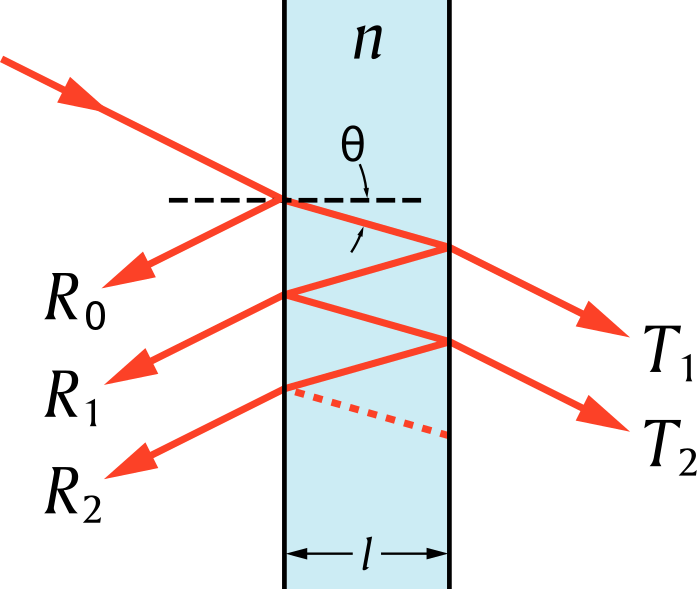
\includegraphics[scale=0.2]{Bilder/FzV/FPI.png}
    \caption{Schematischer Aufbau eines Fabry-Pérot-Interferometer.}
\end{figure}\\
Trifft ein Lichtstrahl unter dem Einfallswinkel $\alpha$ auf die erste Grenzfläche 
so wird dieser größtenteils transmittiert. Allerdings wird dieser Strahl an der zweiten 
Grenzfläche mehr reflektiert und nur ein Teil transmittiert. Bei jeder Teilreflektion tritt 
ein kleiner Teil aus. 
Dieser Vorgang ist beliebig oft wiederholbar. 
Letztlich interferieren die entweichenden Lichtstrahlen. 
Wenn diese Teilstrahlen konstruktiv interferieren, wird das Interferometer durchlässig und 
wenn sie destruktiv interferieren, undurchlässig. Wie sie interferieren ist abhängig von 
der Wellenlänge und dem Einfallswinkel. Die Transmission wird mithilfe der Airy-Funktionen beschrieben. \citep[vgl.][]{fpi}
\newpage
\textbf{Konfokales FPI}\\
Bei einem konfokalen FPI werden anstatt den beiden plan-parallelen Spiegeln zwei sphärische Spiegel verwendet.
Der Vorteil eines konfokalem FPI gegenüber einen plan-parallelen ist, dass die Justierung nicht unbedingt exakt sein muss, damit die 
Strahlen nicht aus dem Interferometer hinauslaufen. Dies hat zur Folge, dass die durchgelassene Intensität und Finesse steigt.\\
Wie bereits erläutert wird beim FPI Vielstrahlinterferenz verwendet, um ein Interferenzbild zu erzeugen. 
Die Bedingung für ein Interferenzmaxima lautet:
\begin{equation}
    k \lambda = 2nd \cos(\alpha)
\end{equation}
Wobei $k$ für eine beliebige natürlich Zahl, $n$ für den Brechungsindex und $d$ für den Abstand zwischen den Spiegeln steht.
Weitere wichtige Kenngrößen werden im Folgenden erläutert.\\\\
Eine wichtige Größe ist der \textbf{freie Spektralbereich FSR}. Dieser gibt an wie weit die Maxima verschiedener Beugungsordnungen
noch voneinander getrennt werden können. 
Der freie Spektralbereich ist im Frequenzraum, bei senkrechtem Einfall ($\alpha = 0$) wie folgt definiert:
\begin{equation}
    \Delta \nu_{FSR} = \frac{c}{2 n d }
\end{equation}
Man erkennt, dass der freie Spektralbereich im Frequenzraum konstant ist. Somit kann man bei gleichbleibenden Brechungsindex
sagen, dass der FSR nur vom Abstand der Spiegel abhängig ist. Was im Umkehrschluss bedeutet, dass es einen Zusammenhang
zwischen der messbaren Wellenlänge $\lambda$ 
und dem Abstand $d$ der Spiegel gibt.\\
Ein weiterer wichtiger Parameter ist die \textbf{Finesse}, sie gibt an wie viele Linien im freien Spektralbereich aufgelöst werden können
und ist wie folgt definiert:
\begin{equation}
    F = \frac{\Delta \nu_{FSR}}{\Delta \nu}
\end{equation}
Wobei $\Delta \nu$ für die Halbwertsbreite der Maxima steht. \cite[vgl.][]{fpi2}\\
Das nachfolgende Bild zeigt ein Transmissionsspektrum eines FPI.
\begin{figure}[h]
    \centering
    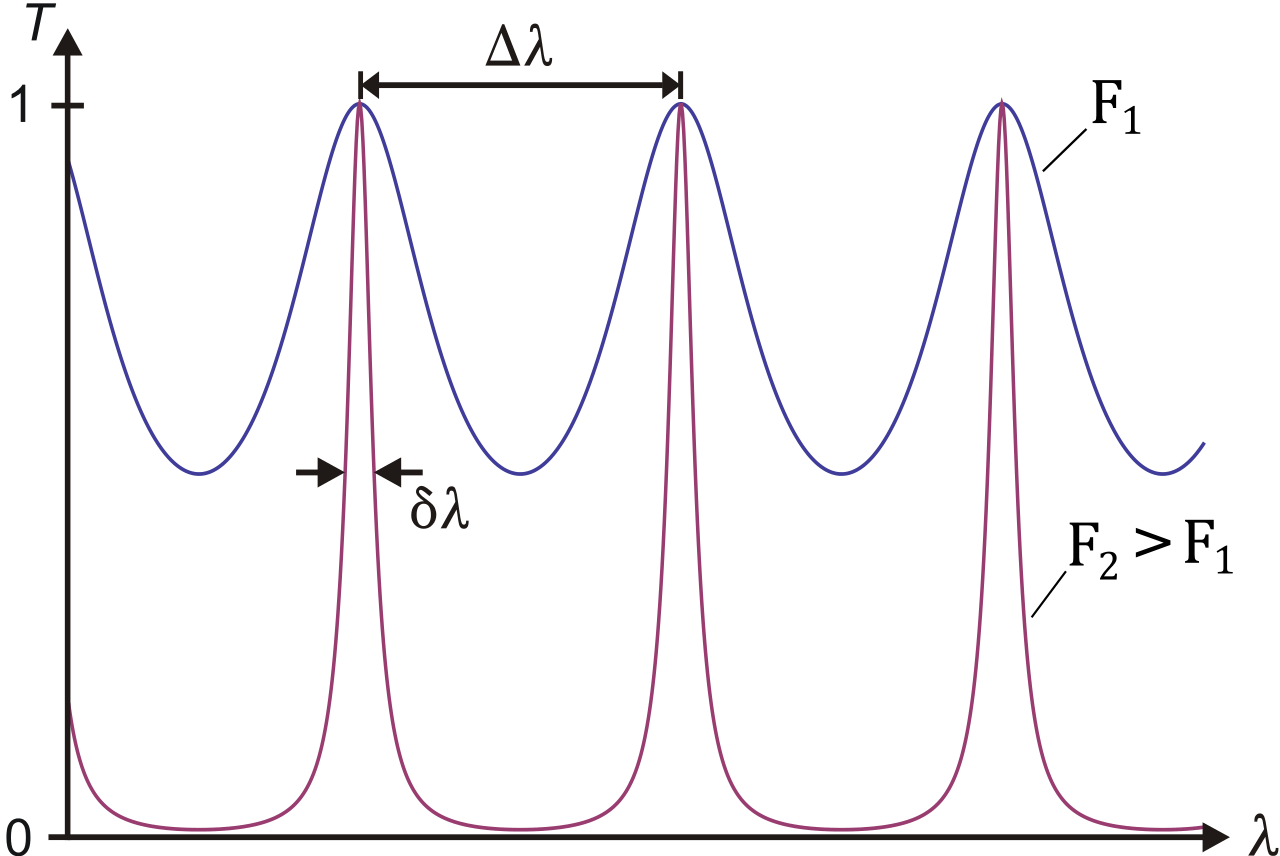
\includegraphics[scale=0.2]{Bilder/FzV/FPI2.png}
    \caption{Beispielhaftes Transmissionsspektrums eines Fabry-Pérot-Interferometer für zwei unterschiedlichen Finessen.}
\end{figure}\\
Hier sind zwei Graphen 
dargestellt, der eine Graph zeigt ein Transmissionsspektrum für eine ‚gute‘ Finesse (rot) 
und der zweite zeigt den Verlauf für eine schlechtere Finesse (blau). 
Die Finesse eines Interferometers sollte möglichst groß sein, damit die Beugungsordnungen gut voneinander trennbar sind. 
In dieser Graphik wird der freie Spektralbereich nicht im Frequenzraum dargestellt, sondern mithilfe der Wellenlänge ($\Delta \lambda$) 
und die Halbwertsbreite der Interferenzmaxima wird in der Graphik als $\delta \lambda$, 
ebenfalls abhängig von der Wellenlänge, gekennzeichnet. \citep[vgl.][]{fpi1}
